\documentclass[12pt]{article}
%\usepackage{times}
\usepackage{cite}
\usepackage{indentfirst}
\usepackage{subcaption}
\usepackage{graphicx}
%this is a comment
\title{Volunteer Connector - Software Requirements and Planning}
\author{Daniel Domme (onid: dommed), \\
Charles Koll (onid: kollch), \\
Pedro Autran e Morais (onid: autranep), \\
Coulby Nguyen (onid: nguyenco), \\
Pavel Shonka (onid: shonkap)
}
\date{29 January 2018}

\begin{document}
\maketitle
%\tableofcontents

\section{Project Description}
Nothing can quite match the feeling of volunteering one's time or donating items to those
in need. Communities and individuals alike receive positive benefits \cite{vol} and are
connected more closely. Unfortunately, there will always be a need for volunteers to help
charitable organizations, and there are some challenges in meeting those needs. For
potential volunteers, there is a severe lack of a central website to look for the right
opportunities suited for them. It can be hard to know where to start to look or to even
think of what they might like devoting their time to. For charities, advertising costs can
be prohibitive, and there is no obvious place to provide information for the needs that
they have. The solution to this is a central website that allows charitable organizations
to post advertisements for events and volunteer positions that will allow people in the
community to search and connect with them.

The chosen approach is a website that is similar to a job posting board. Charities will
have a special account that allows them to create postings advertising their needs, and it
will be searchable for volunteer position type, organization name, and location. The
intended users are ordinary people in the community and charitable organizations and
events. A big feature that will set this website apart from others is that our services
will be free for the users. There will be no cost for posting advertisements. We are not
trying to turn charity into profit.

The website will be designed using PHP as the structure, CSS for the styling, and
JavaScript for website functionality. This is currently how websites are built and run.
SQL will be used for a database that will contain advertising postings and user accounts.
SQL is currently one of the database languages taught at Oregon State University. Nodejs
will be used to serve up webpages because it is open source and free with many modules and
libraries and is dynamic. \cite{volwebsite}

To help users of the website, there will be an about page to give information on the
website and its functions. Along with this, instructions will be provided for all
functions in a clear manner using text.

A major feature of this website that helps it be effective is that it is free to all
users. Charities will not be forced to pay in order to post. Another feature is that it
will be simple to use and very intuitive. There won't be overcrowding and advertisements.
Thirdly, the site's postings will be highly searchable for the users. It will be easy for
potential volunteers to find what they want. The final major feature is that there are
only two types of users. This makes it simple and clear what abilities you have, and it
reduces risks for the users by limiting actions available.

A feature that we hope to implement is more basic user account customizability. We would
like to let the users save search options and make a unique profile. Another feature that
we are hopeful for is being able to take donations to cover server and bandwidth costs.
\subsection{Functional Requirements}
\begin{enumerate}
\item
	The website will have two types of user accounts. The first account will be of
	charitable organization type with permissions to post advertisements. The second
	account will be of user type that will only be able to search and save postings.
\item
	Advertisement forms for submittal will have a field for key terms/tags that will
	aid in searching postings. They will also have a field for a description of the
	type of activity, location of work by city and state, address, and charitable
	organization name.
\item
	Before advertisements may be submitted, all blank fields must be filled out.
\item
	Charitable organizations will have the option to delete or edit their
	advertisements.
\item
	Volunteer opportunity advertisements must be searchable. Searches will be able to
	be refined by location, charities, and keywords.
\item
	The home page will have a search bar, login button, register button, navigation
	bar, and location changer.
\item
	An about page will provide information on the website and its functions.
\end{enumerate}
\subsection{Nonfunctional Requirements}
\begin{enumerate}
\item
	The website should support mobile devices and small screens.
\item
	All browsers should be supported by the site.
\item
	Navigation through the site should be intuitive and clear.
\item
	Users should be able to favorite posts easily with the click of a button.
\item
	Feedback should be given when posts are completed and added to the database.
\item
	Functions of the website should be clear with helpful instructions and feedback.
\end{enumerate}
\section{Use Cases}
\subsection{Post Volunteer Inquiry}
\subsubsection{Goal}
allow charity organizations to post their volunteer needs for the public to see
\subsubsection{Actor}
Charity Event Organizer
\subsubsection{Preconditions}
\begin{itemize}
\item
	The charity event/activity has already been planned and scheduled with a date,
	time, and location
\item
	The Organizer is at the login menu
\item
	Charity Event Organizer knows how many volunteers he/she is asking for/requiring
\end{itemize}
\subsubsection{Postconditions}
\begin{itemize}
\item
	Event listing is posted to the website for volunteers to see and are able to
	register
\end{itemize}
\subsubsection{Flow of Events}
\begin{itemize}
\item
	Event Organizer enters charity account username and password
\item
	Website application verifies the credentials and logs organizer in with the
	abilities to post new event listings
\item
	Event Organizer clicks the 'add event listing' button and a modal pops up, the
	organization's name is autofilled based on the account
\item
	The modal prompts the Organizer to enter the event name, a short event
	description, volunteer type, number of volunteers needed, date, and lastly
	location
\item
	The organizer clicks the 'add post' button at the bottom of the modal, the modal
	disappears, and a text box that says post successfully posted appears at the top
	of the screen
\item
	The post is now on the feed of charity event postings
\end{itemize}
\subsubsection{Quality Requirements}
\begin{itemize}
\item
	The post is posted to the postings feed no later than 1 minute after the organizer
	has clicked the 'add post' button
\end{itemize}
\subsection{Volunteer Event Registration}
\subsubsection{Goal}
have volunteer users register for events posted by charity organizations
\subsubsection{Actor}
Volunteering Citizen
\subsubsection{Preconditions}
\begin{itemize}
\item
	The user has an account that has their basic information: name, age, and location
\item
	The user is at the login menu
\item
	The user has an intent to volunteer
\end{itemize}
\subsubsection{Postconditions}
\begin{itemize}
\item
	The user has been registered to attend the event they are interested in
\end{itemize}
\subsubsection{Flow of Events}
\begin{itemize}
\item
	The user enters his/her account username and password
\item
	The user selects the event he/she is interested in
\item
	Then the user reads through the information to understand the details of the
	specific volunteer work
\item
	Next the user clicks the 'volunteer' button of that post
\item
	This automatically adds this user information to this events personnel
\item
	A text box appears saying that they have successfully registered for 'x' event
\end{itemize}
\subsubsection{Quality Requirements}
\begin{itemize}
\item
	If the event is cancelled the user is known within 30 minutes of that cancellation
\item
	When the user hits 'volunteer' they are added to that post's data within a minute
\end{itemize}
\subsection{User search for an event}
\subsubsection{Goal}
have the volunteer users be able to search for an event
\subsubsection{Actor}
Volunteering Citizen
\subsubsection{Preconditions}
\begin{itemize}
\item
	The user has already been logged in
\item
	They have a search inquiry in mind
\end{itemize}
\subsubsection{Postconditions}
\begin{itemize}
\item
	Displays all the results tha pertain to the user's search inquiry
\end{itemize}
\subsubsection{Flow of Events}
\begin{itemize}
\item
	The user is in the search menu
\item
	The search menu prompts the user to enter a keyword into the search bar
\item
	The user enters the keyword of the event they are looking for
\item
	The search menu prompts the user if they want to limit the search based on
	location
\item
	The user selects what they wish and presses search
\item
	This displays all of the events with the specified information given by the user
\end{itemize}
\subsubsection{Quality Requirements}
\begin{itemize}
\item
	The event posts that match the requirements should be displayed no later than 30
	seconds after the user hits the 'search' button
\end{itemize}
\subsection{Overview}
These three cases cover the most important aspects of our program: number one, charity
organizations creating posts about their events and about how many volunteers they need to
run, operate, and help at that event; number two, volunteer users reading the full event
information, finding out what the date and where the location of the event is and
registering to help for that event if the event criteria matches their own needs; and
lastly, the volunteer user search functionality, so that it is easier to find events that
meet a user's criteria, instead of scrolling through the event feed until they find an
event that fits.

One clear error scenario that could arise would be that are not enough volunteer users,
therefore charity organizations won't post events since it would be pointless due to
nobody registering for their events. This problem can be remedied in a couple different
ways, starting with advertising the app to current volunteer groups to get that audience
involved with the application. Another option would be to partner with big charity
organizations and have all of their events run through the application.
\section{Planning}
\subsection{Milestones/Tasks}
\begin{itemize}
\item
	Deciding database structure
	\begin{itemize}
	\item
		Dependencies: none
	\end{itemize}
\item
	Deciding layout of site
	\begin{itemize}
	\item
		Dependencies: none
	\end{itemize}
\item
	Build basic HTML of site
	\begin{itemize}
	\item
		Dependencies: layout of site
	\end{itemize}
\item
	Build database
	\begin{itemize}
	\item
		Dependencies: database structure
	\end{itemize}
\item
	Write Nodejs that queries database for data
	\begin{itemize}
	\item
		Dependencies: database structure, layout of site, database
	\end{itemize}
\item
	Improve look of site with CSS
	\begin{itemize}
	\item
		Dependencies: layout of site, basic HTML
	\end{itemize}
\item
	Add maneuverability features with JavaScript
	\begin{itemize}
	\item
		Dependencies: layout of site, basic HTML, Nodejs for data
	\end{itemize}
\item
	Repeat last two tasks (CSS and JavaScript) until complete
\end{itemize}
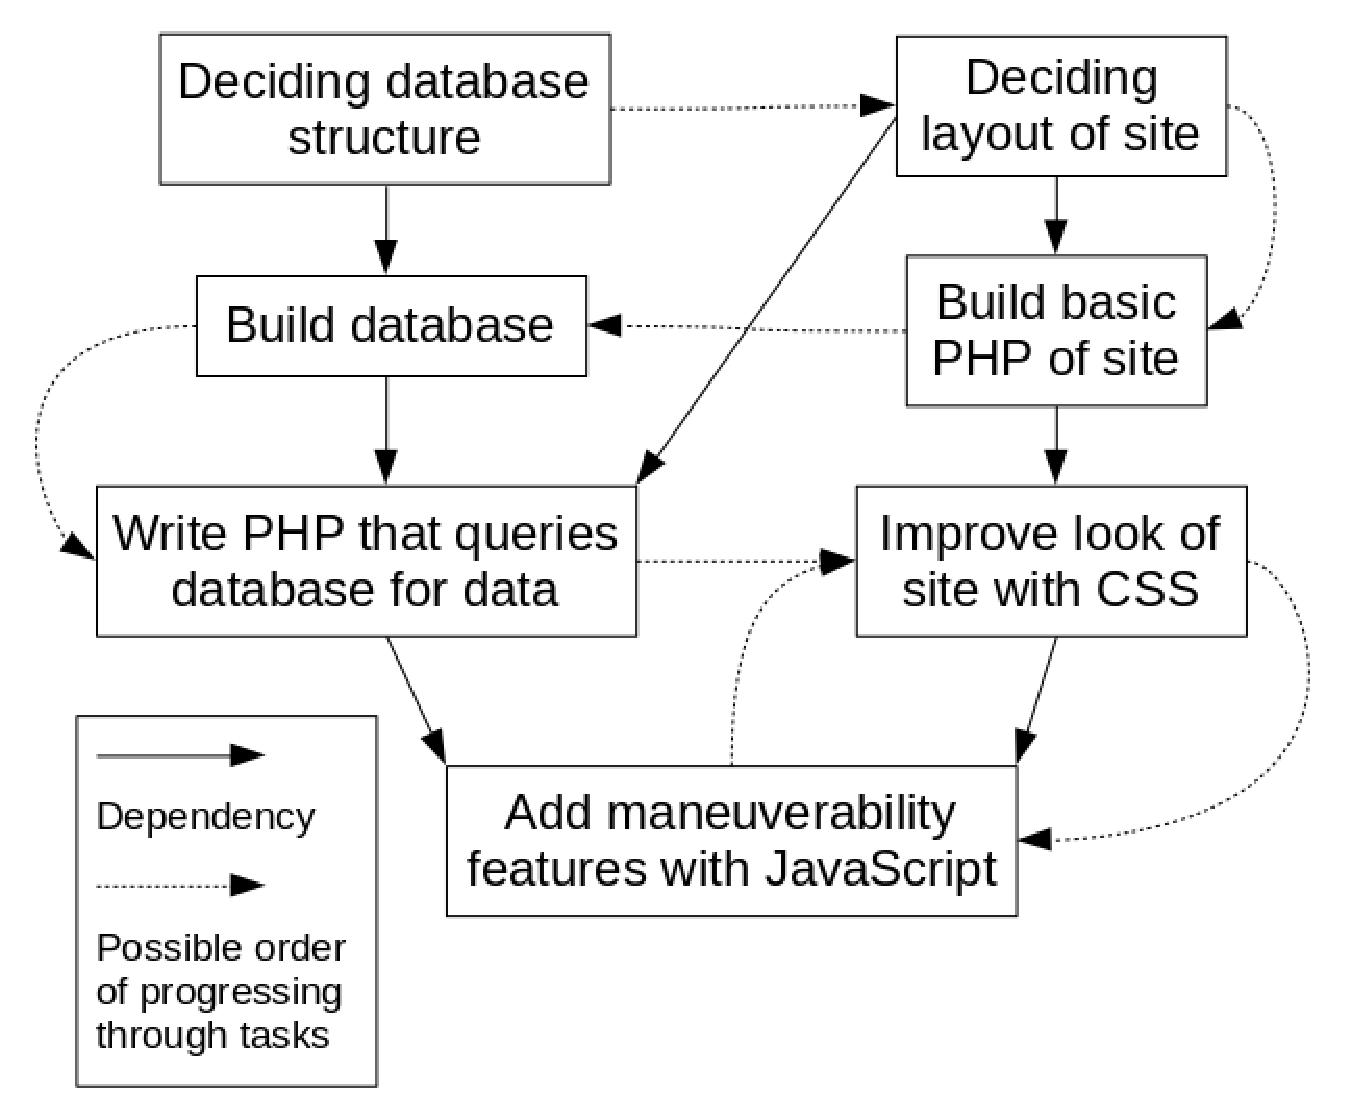
\includegraphics[width=\textwidth]{task_flowchart}
The tasks have been ordered in such a way that they aren't done before any of their
dependencies. In addition, they are laid out so that the front-end and back-end can be
done concurrently for the most part.
\subsection{Resources for the tasks}
\subsubsection{Deciding database structure}
Group members sketching out the structure on a piece of paper is the only requirement, but
a software program such as ERDPlus can ease the process of designing
\subsubsection{Deciding layout of site}
Group members sketching on a piece of paper
\subsubsection{Build basic HTML of site}
Computer to write code on and test
\subsubsection{Build database}
Server to host database, computer to access server
\subsubsection{Write PHP that queries database for data}
Computer to write PHP on and test, internet connection to access the server
\subsubsection{Improve look of site with CSS}
Computer to write CSS on and test, internet connection to access the server
\subsubsection{Add maneuverability features with JavaScript}
Computer to write JavaScript on and test, internet connection to access the server
\subsection{Schedule/Timeline}
\begin{tabular}{|p{1in}|p{1in}|p{1in}|p{1in}|} \hline
	& Server Team & Database Team & Frontend Team \\ \hline
	Week 1 & Choose what backend features to use (templates etc) & Decide layout of
	database & Design a UI and draft up some designs \\ \hline
	Week 2 & Start writing server code, landing page, user profiles & Start writing
	database schema & Decide on a UI and begin implementing UI in HTML \\ \hline
	Week 3 & Continue writing server code, search functions, navigation between pages
	& Make decisions on what functionality and information to store & Add CSS/styling
	to UI \\ \hline
	Week 4 & Implement user profiles, connect with database & Optimize database, help
	out other teams & Iterate on CSS/styling, prototype client-side interaction \\
	\hline
	Week 5 & & & Add frontend interaction/javascript \\ \hline
\end{tabular}
\subsection{Project tracking}
The project will be developed using Git. This not only allows for revision control, but
also for the ability to easily break up the project into sections. To do this, we will
make each task its own branch. Doing so allows for the project to be viewed as features,
as well as making it easy for different people to do different tasks. This will also help
keep the project modular and allow us to separate concerns and share work when necessary.
In our sub-weekly meetings we can evaluate the pace of our project. In addition, we will
create and follow a gantt chart to give us an estimate of the goals we should be hitting
and when.
\subsection{Risk Management}
\subsubsection{Risk 1: Not enough time to complete all functionality}
This would be the case if the project is too feature-intense to be completed in the
allotted time by only 5 people. To mitigate this risk, our weekly meetings should discuss
workload. If we feel workload is getting unmanageable, we should discuss as a group what
the most important/minimal features are for basic functionality, and reduce the scope of
the project so we can at least complete this core functionality. Iterate as needed.
\subsubsection{Risk 2: Not following pre-built plans}
If a team or group does not follow the plans correctly due to miscommunications this can
lead to a lot of wasted work or to some teams taking up tasks that are not reasonable to
complete in the allotted time. To minimize this risk, we can do group code reviews to see
that each group is doing what is expected of them by the other groups.
\subsubsection{Risk 3: Some teams are given too much work and others are not given enough}
This may happen since teams are split up by type of work which may not reflect quantity of
work. It will be useful to make sure each team is prepared to contribute to other teams'
subprojects and have weekly progress meetings about the subprojects. If one team finishes
something early, we should decide as a group if they should move onto their next task or
help another team out.
\section{Meeting Report}
This week we met with the customer and went over what we needed to do for assignment 2. We
also got the description for what the customer wanted for the project and wrote that down.
Things we might not be able to complete in time were also brought up. Hopefully next week
we will be able to figure out exactly how we want the website to function and a base idea
for what it will look like. After deciding what we think we will be able to complete in
the time frame, we will go over the full design and functionality with the customer one
more time before we begin building the website.
\subsection{Team member contribution}
Daniel Domme: Project Description

Coulby Nguyen: Use Cases

Charles Koll: Planning

Pavel Shonka: Meeting Report

Pedro Autran e Morais: Planning

\bibliography{myref}
\bibliographystyle{unsrt}

\end{document}
